\section{Exercice 11 - Coloration des sommets d'un graphe et coloration des arêtes d'un graphe}

Un graphe est $2-$coloriable si et seulement si il est possible de partitionner ce dernier en deux
ensembles stables. Un graphe 2-coloriable est donc un graphe biparti, or le problème de décider si
un graphe est biparti est un problème polynomial, le problème de la $2-$coloration est donc un
problème polynomial.

Un graphe est $2-$arête$-$coloriable s'il l'ensemble $V$ de ses arêtes est divisible en deux ensembles
$F$ et $E$ distincts vérifiant :
\begin{enumerate}
	\item $E \cup F = V$
	\item $E \cap F = \emptyset$
	\item $\forall ((i,j), (k,l)) \in E^2, \quad i \not = k, \not = l, j \not = k, j \not = l$
	\item $\forall ((i,j), (k,l)) \in J^2, \quad i \not = k, \not = l, j \not = k, j \not = l$
\end{enumerate}

$E$ et $F$ sont alors des couplages de $G$. Un algorithme résolvant ce problème consiste en la
recherche d'un couplage maximum $C$ puis en vérifiant que $V \ C$ est aussi un couplage. Si tel est
le cas, le graphe est $2-$arête$-$coloriable. 

La recherche d'un couplage se faisant en temps polynomial, l'algorithme énoncé ci-dessus est
polynomial.

\section{Exercice 12 - Coloration des sommets d'un graphe}

\subsection{Appartenance à $NP$}

\begin{enumerate}
	\item COLOR : \\
		Considérons une solution, un moyen de tester s'il s'agit d'une solution réalisable est de tester
		pour chacun des sommets si ses voisins sont d'une couleur différente en gardant le s couleurs
		rencontrées en mémoire afin de vérifier que leur nombre n'excède pas $k$. La vérification se
		fait alors en $O(n^2)$ et est donc polynomiale.
	\item 3-COLOR : \\
		On procède de la même manière que pour COLOR en s'assurant que le nombre de couleur ne dépasse
		pas $3$, la vérification est alors aussi polynomiale
	\item 3-COLOR-PLAN : \\
		La vérification de la validité de la $3-$coloration se fait comme précédemment en $O(n^2)$. Il
		fait cependant tester si le graphe est planaire qui est un problème polynomial, la vérification
		est don cpolynomiale.
\end{enumerate}

Tous ces problèmes appartiennent donc à $NP$.

\subsection{Relation enre 3-COLOR et COLOR}

Supposons qu'il existe un algorithme résolvant COLOR en temps polynomial quelque soit $k$, il existe
alors un algorithme polynomial résolvant 3-COLOR. Par contraposition, on vient de démontrer que si
3-COLOR est $NP$-difficile alors COLOR est $NP$-difficile.

\subsection{Étude du problème COLOR}

\subsubsection{Graphe $G_{\phi}$}

\begin{center}
	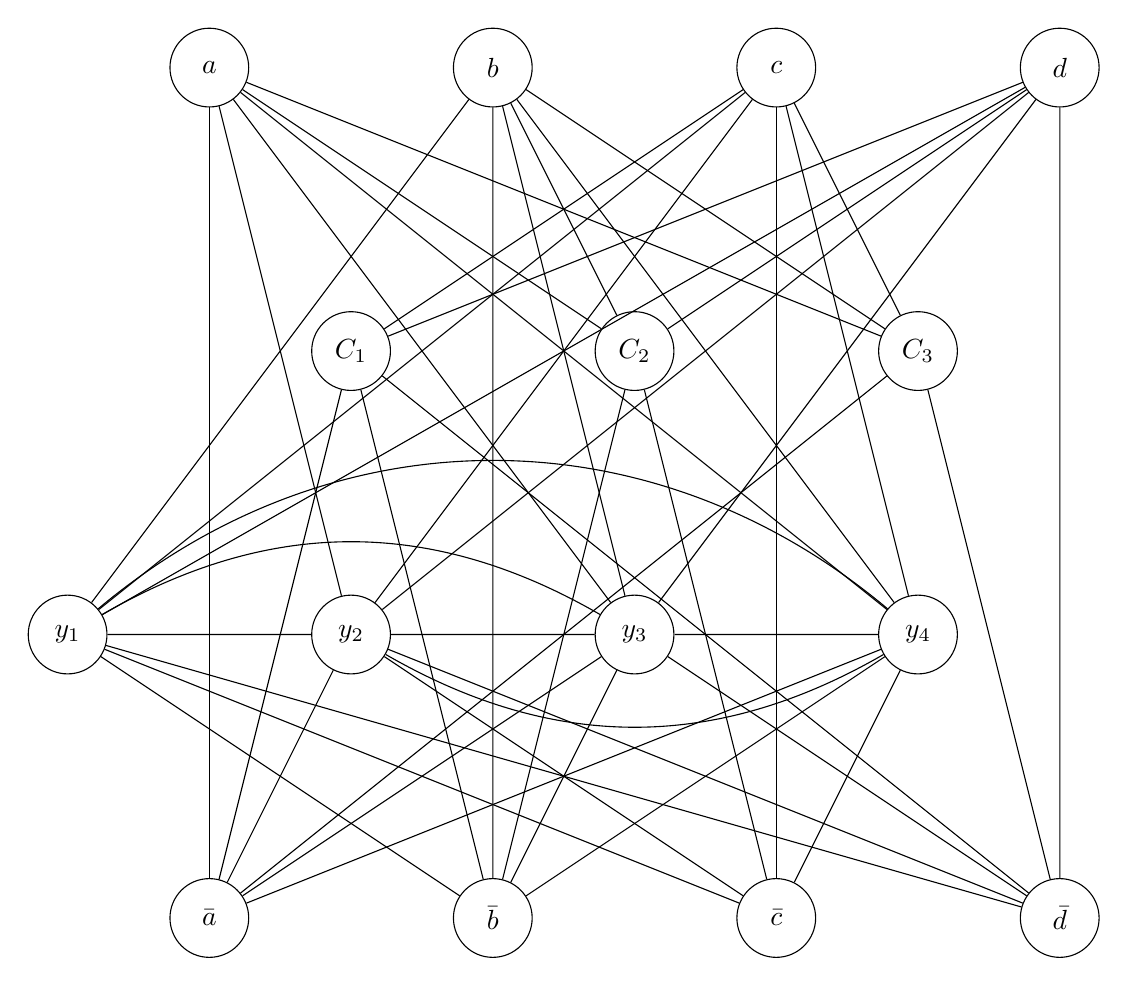
\begin{tikzpicture}[scale=1.8]
		\tikzset{nd/.style={circle, draw=black, minimum width=1cm}};
		\node[nd] (a) at (2, 6) {$a$};
		\node[nd] (b) at (4, 6) {$b$};
		\node[nd] (c) at (6, 6) {$c$};
		\node[nd] (d) at (8, 6) {$d$};
		\node[nd] (na) at (2, 0) {$\bar a$};
		\node[nd] (nb) at (4, 0) {$\bar b$};
		\node[nd] (nc) at (6, 0) {$\bar c$};
		\node[nd] (nd) at (8, 0) {$\bar d$};
		\node[nd] (c1) at (3, 4) {$C_1$};
		\node[nd] (c2) at (5, 4) {$C_2$};
		\node[nd] (c3) at (7, 4) {$C_3$};
		\node[nd] (y1) at (1, 2) {$y_1$};
		\node[nd] (y2) at (3, 2) {$y_2$};
		\node[nd] (y3) at (5, 2) {$y_3$};
		\node[nd] (y4) at (7, 2) {$y_4$};

		\draw (a) -- (na);
		\draw (b) -- (nb);
		\draw (c) -- (nc);
		\draw (d) -- (nd);

		\draw (y1) -- (y2);
		\draw (y1) to[out=30, in=150](y3);
		\draw (y1) to[out=40, in=140](y4);

		\draw (y2) -- (y3);
		\draw (y2) to[out=330, in=210] (y4);

		\draw (y3) -- (y4);

		\draw (y1) -- (b);
		\draw (y1) -- (c);
		\draw (y1) -- (d);
		\draw (y1) -- (nb);
		\draw (y1) -- (nc);
		\draw (y1) -- (nd);

		\draw (y2) -- (a);
		\draw (y2) -- (c);
		\draw (y2) -- (d);
		\draw (y2) -- (na);
		\draw (y2) -- (nc);
		\draw (y2) -- (nd);

		\draw (y3) -- (a);
		\draw (y3) -- (b);
		\draw (y3) -- (d);
		\draw (y3) -- (na);
		\draw (y3) -- (nb);
		\draw (y3) -- (nd);

		\draw (y4) -- (a);
		\draw (y4) -- (b);
		\draw (y4) -- (c);
		\draw (y4) -- (na);
		\draw (y4) -- (nb);
		\draw (y4) -- (nc);

		\draw (c1) -- (na);
		\draw (c1) -- (nb);
		\draw (c1) -- (c);
		\draw (c1) -- (d);
		\draw (c1) -- (nd);

		\draw (c2) -- (a);
		\draw (c2) -- (nb);
		\draw (c2) -- (nc);
		\draw (c2) -- (d);
		\draw (c2) -- (b);

		\draw (c3) -- (na);
		\draw (c3) -- (a);
		\draw (c3) -- (b);
		\draw (c3) -- (c);
		\draw (c3) -- (nd);


	\end{tikzpicture}
\end{center}
